\documentclass{standalone}
\usepackage{tikz}
\usetikzlibrary{patterns, positioning}

\begin{document}
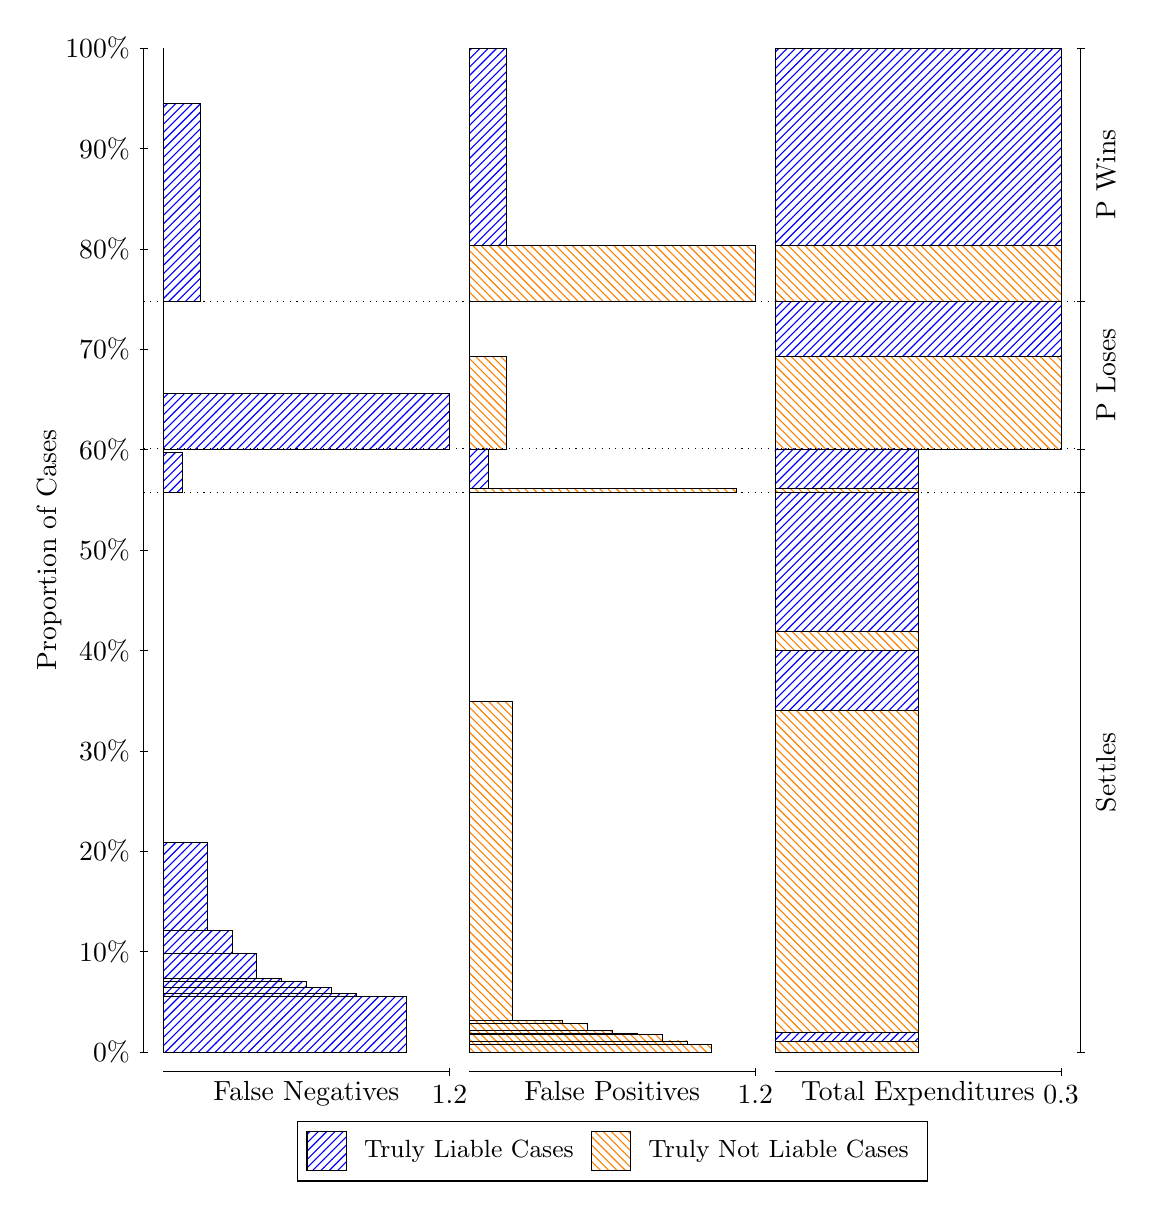
\begin{tikzpicture}
\draw[black, very thin] (1.5,1.75) -- (1.5,14.5);
\node[rotate=90, anchor=center] at (0.3, 8.125) {Proportion of Cases};
\draw[black, very thin] (1.45,1.75) -- (1.55,1.75);
\node[anchor=east] at (1.45, 1.75) {0\%};
\draw[black, very thin] (1.45,3.025) -- (1.55,3.025);
\node[anchor=east] at (1.45, 3.025) {10\%};
\draw[black, very thin] (1.45,4.3) -- (1.55,4.3);
\node[anchor=east] at (1.45, 4.3) {20\%};
\draw[black, very thin] (1.45,5.575) -- (1.55,5.575);
\node[anchor=east] at (1.45, 5.575) {30\%};
\draw[black, very thin] (1.45,6.85) -- (1.55,6.85);
\node[anchor=east] at (1.45, 6.85) {40\%};
\draw[black, very thin] (1.45,8.125) -- (1.55,8.125);
\node[anchor=east] at (1.45, 8.125) {50\%};
\draw[black, very thin] (1.45,9.4) -- (1.55,9.4);
\node[anchor=east] at (1.45, 9.4) {60\%};
\draw[black, very thin] (1.45,10.675) -- (1.55,10.675);
\node[anchor=east] at (1.45, 10.675) {70\%};
\draw[black, very thin] (1.45,11.95) -- (1.55,11.95);
\node[anchor=east] at (1.45, 11.95) {80\%};
\draw[black, very thin] (1.45,13.225) -- (1.55,13.225);
\node[anchor=east] at (1.45, 13.225) {90\%};
\draw[black, very thin] (1.45,14.5) -- (1.55,14.5);
\node[anchor=east] at (1.45, 14.5) {100\%};

\draw[black, very thin] (13.4,1.75) -- (13.4,14.5);
\draw[black, very thin] (13.35,1.75) -- (13.45,1.75);
\node[anchor=west] at (13.35, 1.75) {};
\draw[black, very thin] (13.35,8.8574) -- (13.45,8.8574);
\node[anchor=west] at (13.35, 8.8574) {};
\draw[black, very thin] (13.35,9.4103) -- (13.45,9.4103);
\node[anchor=west] at (13.35, 9.4103) {};
\draw[black, very thin] (13.35,11.281) -- (13.45,11.281);
\node[anchor=west] at (13.35, 11.281) {};
\draw[black, very thin] (13.35,14.5) -- (13.45,14.5);
\node[anchor=west] at (13.35, 14.5) {};

\draw[black, very thin, pattern color=blue, pattern=north east lines] (1.75,1.75) rectangle (4.8304,2.4527);
\draw[black, very thin, pattern color=blue, pattern=north east lines] (1.75,2.4527) rectangle (4.5145,2.455);
\draw[black, very thin, pattern color=blue, pattern=north east lines] (1.75,2.455) rectangle (4.1986,2.4892);
\draw[black, very thin, pattern color=blue, pattern=north east lines] (1.75,2.4892) rectangle (3.8826,2.5729);
\draw[black, very thin, pattern color=blue, pattern=north east lines] (1.75,2.5729) rectangle (3.5667,2.6416);
\draw[black, very thin, pattern color=blue, pattern=north east lines] (1.75,2.6416) rectangle (3.2507,2.6863);
\draw[black, very thin, pattern color=blue, pattern=north east lines] (1.75,2.6863) rectangle (2.9348,2.9974);
\draw[black, very thin, pattern color=blue, pattern=north east lines] (1.75,2.9974) rectangle (2.6188,3.2904);
\draw[black, very thin, pattern color=blue, pattern=north east lines] (1.75,3.2904) rectangle (2.3029,4.4075);
\draw[black, very thin, pattern color=orange, pattern=north west lines] (1.75,4.4075) rectangle (1.75,8.8574);
\draw[black, very thin, pattern color=blue, pattern=north east lines] (1.75,8.8574) rectangle (1.987,9.3624);
\draw[black, very thin, pattern color=orange, pattern=north west lines] (1.75,9.3624) rectangle (1.75,9.4103);
\draw[black, very thin, pattern color=blue, pattern=north east lines] (1.75,9.4103) rectangle (5.3833,10.111);
\draw[black, very thin, pattern color=orange, pattern=north west lines] (1.75,10.111) rectangle (1.75,11.281);
\draw[black, very thin, pattern color=blue, pattern=north east lines] (1.75,11.281) rectangle (2.2239,13.793);
\draw[black, very thin, pattern color=orange, pattern=north west lines] (1.75,13.793) rectangle (1.75,14.5);
\draw[black, very thin, pattern color=orange, pattern=north west lines] (5.6333,1.75) rectangle (8.7138,1.8504);
\draw[black, very thin, pattern color=orange, pattern=north west lines] (5.6333,1.8504) rectangle (8.3978,1.8914);
\draw[black, very thin, pattern color=orange, pattern=north west lines] (5.6333,1.8914) rectangle (8.0819,1.9691);
\draw[black, very thin, pattern color=orange, pattern=north west lines] (5.6333,1.9691) rectangle (7.7659,1.9866);
\draw[black, very thin, pattern color=orange, pattern=north west lines] (5.6333,1.9866) rectangle (7.45,2.0206);
\draw[black, very thin, pattern color=orange, pattern=north west lines] (5.6333,2.0206) rectangle (7.1341,2.1121);
\draw[black, very thin, pattern color=orange, pattern=north west lines] (5.6333,2.1121) rectangle (6.8181,2.1518);
\draw[black, very thin, pattern color=orange, pattern=north west lines] (5.6333,2.1518) rectangle (6.5022,2.1531);
\draw[black, very thin, pattern color=orange, pattern=north west lines] (5.6333,2.1531) rectangle (6.1862,6.1998);
\draw[black, very thin, pattern color=blue, pattern=north east lines] (5.6333,6.1998) rectangle (5.6333,8.8574);
\draw[black, very thin, pattern color=orange, pattern=north west lines] (5.6333,8.8574) rectangle (9.0297,8.9052);
\draw[black, very thin, pattern color=blue, pattern=north east lines] (5.6333,8.9052) rectangle (5.8703,9.4103);
\draw[black, very thin, pattern color=orange, pattern=north west lines] (5.6333,9.4103) rectangle (6.1072,10.58);
\draw[black, very thin, pattern color=blue, pattern=north east lines] (5.6333,10.58) rectangle (5.6333,11.281);
\draw[black, very thin, pattern color=orange, pattern=north west lines] (5.6333,11.281) rectangle (9.2667,11.989);
\draw[black, very thin, pattern color=blue, pattern=north east lines] (5.6333,11.989) rectangle (6.1072,14.5);
\draw[black, very thin, pattern color=orange, pattern=north west lines] (9.5167,1.75) rectangle (11.333,1.8825);
\draw[black, very thin, pattern color=blue, pattern=north east lines] (9.5167,1.8825) rectangle (11.333,2.0027);
\draw[black, very thin, pattern color=orange, pattern=north west lines] (9.5167,2.0027) rectangle (11.333,6.0835);
\draw[black, very thin, pattern color=blue, pattern=north east lines] (9.5167,6.0835) rectangle (11.333,6.8549);
\draw[black, very thin, pattern color=orange, pattern=north west lines] (9.5167,6.8549) rectangle (11.333,7.0915);
\draw[black, very thin, pattern color=blue, pattern=north east lines] (9.5167,7.0915) rectangle (11.333,8.8574);
\draw[black, very thin, pattern color=orange, pattern=north west lines] (9.5167,8.8574) rectangle (11.333,8.9052);
\draw[black, very thin, pattern color=blue, pattern=north east lines] (9.5167,8.9052) rectangle (11.333,9.4103);
\draw[black, very thin, pattern color=orange, pattern=north west lines] (9.5167,9.4103) rectangle (13.15,10.58);
\draw[black, very thin, pattern color=blue, pattern=north east lines] (9.5167,10.58) rectangle (13.15,11.281);
\draw[black, very thin, pattern color=orange, pattern=north west lines] (9.5167,11.281) rectangle (13.15,11.989);
\draw[black, very thin, pattern color=blue, pattern=north east lines] (9.5167,11.989) rectangle (13.15,14.5);
\draw[black, dotted] (1.5,8.8574) -- (13.4,8.8574);
\draw[black, dotted] (1.5,9.4103) -- (13.4,9.4103);
\draw[black, dotted] (1.5,11.281) -- (13.4,11.281);
\draw[black, very thin] (1.75,1.5) -- (5.3833,1.5);
\node[anchor=north] at (3.5667, 1.5) {False Negatives};
\draw[black, very thin] (5.3833,1.45) -- (5.3833,1.55);
\node[anchor=north] at (5.3833, 1.45) {1.2};

\draw[black, very thin] (5.6333,1.5) -- (9.2667,1.5);
\node[anchor=north] at (7.45, 1.5) {False Positives};
\draw[black, very thin] (9.2667,1.45) -- (9.2667,1.55);
\node[anchor=north] at (9.2667, 1.45) {1.2};

\draw[black, very thin] (9.5167,1.5) -- (13.15,1.5);
\node[anchor=north] at (11.333, 1.5) {Total Expenditures};
\draw[black, very thin] (13.15,1.45) -- (13.15,1.55);
\node[anchor=north] at (13.15, 1.45) {0.3};

\node[black, centered, rotate=90] at (13.72, 5.3037) {Settles};

\node[black, centered, rotate=90] at (13.72, 10.346) {P Loses};
\node[black, centered, rotate=90] at (13.72, 12.891) {P Wins};

\draw (7.449999999999999,1.5) node[draw=none] (baseCoordinate) {};
\begin{scope}[align=center]
        \matrix[scale=0.5, draw=black, below=0.5cm of baseCoordinate, nodes={draw}, column sep=0.1cm]{
            \node[rectangle, draw, minimum width=0.5cm, minimum height=0.5cm, pattern=north east lines, pattern color=blue] {}; &
            \node[draw=none, font=\small] (B) {Truly Liable Cases}; &
            \node[rectangle, draw, minimum width=0.5cm, minimum height=0.5cm, pattern=north west lines, pattern color=orange] {}; &
            \node[draw=none, font=\small] (B) {Truly Not Liable Cases}; \\
            };
\end{scope}

\end{tikzpicture}
\end{document}